\myChapter{Service Oriented Architecture for EAs}\label{chap:soaea}
\minitoc\mtcskip
\vfill
\lettrine{S}{OA} provides a good set of solutions to solve some of the problems in the EA area, such as the lack of integration, standardization and dynamism control. It also allows ease of development in dynamic, distributed and heterogeneous systems. However, several restrictions must be taken into account. In this chapter, we present the existent restrictions in the EA design, according to WHATEVER. Also, the restrictions in SOA design (such as the unordered execution or distribution transparency) are explained to perform a good design of services for EAs. All these requirements are used to explain how the different elements of an EA must be designed.

SOMA methodology \cite{Arsanjani2008SOMA}, explained in previous chapter, establish that the phases of the SOA design are {\em identification}, {\em specification} and {\em realization} of the services and flows. In this chapter we identify the services that compose an EA and specify some of their possible behaviours. The realization of the designed services will be explained, using an specific technology, in next chapter. 

For a better understanding, a complete example of development of an EA is explained. This example is modified to show how to convert an algorithm to another, dynamic operator changing, load balancing and even intelligent aggregation of operators.

\section{Design of services for Evolutionary Algorithms}

This section shows the restrictions for designing EAs (from the point of view of a EA practitioner) and services (from the SOA area expertise).

\subsection{Restrictions in EAs design}

%%%PONER LO GENERICITY DE PAPAZOGLOU
The work of \person{Gagn\'e and Parizeau} \cite{GENERICITY05} established six criteria to qualify the genericity of a framework for EAs. 

\begin{itemize}
\item Generic representation: independence of the structure of the individuals. Therefore, services must accept {\em Individuals} interfaces as inputs, not concrete implementations (such as vectors or lists).

\item Generic fitness: 

\item Generic operations

\item Generic evolutionary model 

\item Parameter management

\item Configurable output
\end{itemize}

\subsection{Restrictions in SOA design}

SOA follows these lines of genericity presented in previous sub-section, and can also extend them:
\begin{itemize}
\item Genericity in the service interfaces: service interfaces are established to create new implementations. Furthermore, these interfaces must be abstract enough to avoid their modification.
\item Programming language independence: for example, services implemented in Java can use services implemented in C++ and vice-versa.
\item Distribution transparency: it is not mandatory to use a specific library for the distribution, or modify the code to adapt the existing operators.
\item Flexibility: easy to add and remove elements to use the self-adaptation or other mechanisms.
\end{itemize}

As explained in previous chapter, when developing within a SOA, \cite{Papazoglou2007SOA} established that the services must be: 
\begin{itemize}
\item Abstract: many different implementations can use the same interface.
\item Well-defined: the interface of the service must be fixed, and it can not change in time, because the consumers or implementations of this interface should be modified with it.
\item Encapsulated: services can use other services, but only the interface should be used to consume a service.
\item Reusable: services should be designed to be used by as many applications as possible. 
\end{itemize}

One of the main restrictions in SOA, apart from focusing in develop abstract services, is the stateless nature of services. Therefore, in SOA the services design must follow several guidelines.

First, as services are unaware of others, there must not be global variables in any part of the code. Services are listening, and waiting to be executed. For example, a fitness service with a counter that is increased each time is called (to stop the algorithm if a limit is reached, for example). If several (and different) algorithms are working in parallel, and calling this function at the same time the counter would not distinguish between algorithms, giving erroneous results. However, a service that maintains some kind of state is allowed, for example, a statistic service that read events from all the algorithms being executed at the same time, but this should be managed to avoid errors.

Also, a service must not be distinguishable from local or remote running in other node in the network. Every stage in the algorithm should be treated as service to be executed in local or in remote, even the {\em Population} or the {\em Parameters}. Mechanisms to ensure the correct data-sharing should be provided. Also, many implementations of the same service could exist at the same time (different implementations of {\em Crossover}, for example) and it should be correctly managed and used.

Moreover, a service is always a request-response function. For example, the fitness calculation must not be a method of the {\em Individual} implementation, but a function that receives a list of individuals and returns a list of the calculated fitness of that individuals. This allow things such as remote fitness calculation and distributed load balancing, impossible to perform if the fitness is a method of the {\em Individual} class.

Thinking as abstract as possible requires separate concepts such the order of recombination, and the crossover itself. Usually, after parent selection, individuals are crossed in order. However, if we need a different mechanism for mating (for example, using more than two parents, or parent selected several times) a duplication of effort is needed. That is the reason we should separate the concept {\em recombine} from {\em crossover} (and also, following the top-down design proposed in SOMA). 

Finally, we must not make assumptions about services previously executed or being executed next. For example, services such {\em Recombinator} or {\em Mutator} should return the individuals with their fitness already calculated. Usually this step is performed in the last stage of the generation, but if we require the individuals for other tasks: for example, a Local Search or a statistics collector to guide the algorithm.

\subsection{Other technological restrictions}

In previous chapter we also presented the advantages of using SOA in Evolutionary Algorithms area: firstly, SOA fits with the genericity advantages in the development of software for EAs \cite{GENERICITY05} and adds new features, like language independence and  distribution mechanisms. It also allows the addition and removal of services in execution time without altering the general execution of the algorithm (that is, it is not mandatory to stop it or to add extra code to support new operators). This issue increases the interoperability between different software elements. Moreover, this allows easy code distribution: SOA does not require the use of a concrete implementation or library.

In this chapter, a new process development, explaining the specific technology used is presented. The services developed must match with the next technological restrictions:
\begin{itemize}
\item These services can dynamically bound to change the needed EA aspects. 
\item The source code of  the basic EA services must not been re-written or re-compiled to achieve this task. 
\item New services can be added in execution time. 
\item No specific source code for a distribution must added, neither the existing source code of the services should be modified for this purpose (that is, changing distribution libraries must not add extra code in existing services).
\end{itemize}

\subsection{Designing the services}

Taking into account the previous restrictions a possible way for designing services for EAs is shown: 

\begin{itemize}
\item Individual representation. Almost all services in an EA (like mutation or selection) will accept individuals as input data and produce/modify these individuals. Due to many kind of individuals may exist, the operators should be as abstract as possible to operate properly.
\item Fitness evaluation. Each problem should implement an interface of the fitness service that receives the individual, allowing the distribution of this service (instead of being a method in the {\em individual} class, for example). However, to be more flexible, the {\em fitness service} must receive a list of at least one individual, to facilitate the parallelism.
\item Definition or addition of every type of operator. Thanks to the loose coupling of services, several crossover or mutation implementations can be created. Moreover, new operators can be added in execution time, without re-compiling the existing ones, or combining them according to several parameters, for example.
\item Adaptation of the evolutionary model. The user can manually select the services to be combined to create a Genetic Algorithm or an Evolution Strategy, for example.
\item Dynamic adaptation of the parameters. Parameters can also be a service, thus the EA developer obtains two advantages: it is not mandatory to distribute the parameters among all services, and also they can be dynamically modified in execution time from an external service, facilitating self-adaptation \cite{eiben2005shared}.
\item Flexible output mechanisms. The developers do not need skills in GUIs (Graphical User Interfaces) or logs programming, because as this kind of services are not coupled to the operators, they can access their information without any modification in the operators.
\end{itemize}






As previously stated, the 
fitness should not be calculated within a method of an Individual class. To be less
coupled, it should be implemented an an external service that receives a list of individuals (facilitating the load balancing). That way, the service is as abstract as possible. Also the parameters should be
a service for the same reason, allowing the possibility of performing
experiments related to the parameter control or tuning \cite{ParameterControlEiben07} in an efficient way
(being separated from the code of the existing operators). Services such as the
{\em recombinator} or the {\em mutator} should not receive one or two
individuals, since not all EAs have the same behaviour. They should receive a
list of individuals to be crossed or mutated each generation. On the other way,
{\em population} should not be a list of individuals: it should be a service
to access the individuals and allow the variation of its structure (for example, a change
from an unique population to a distributed island model) without
affecting  the rest of the pieces of the algorithm. So, other services
external to the EA could consult the {\em population} state and act
accordingly to some rules. 

Using the previous indications as a base, SOA-EA has been created. SOA-EA is an
abstract architecture to develop service oriented EAs, independently
of the technology to be used. Table \ref{tab:reasons} shows some reasons to
migrate to SOA and how services in SOA-EA should be designed. 





\begin{SCtable}[][t]

\resizebox{11cm}{!}{
\begin{tabular}{p{2cm}p{2.5cm}p{3cm}p{7cm}}
%\begin{tabular}{llll}
%\noalign{\smallskip}\hline\noalign{\smallskip}
\hline
\rowcolor{colorCorporativoSuave}\textbf{Element} & \textbf{Current EAs development} & \textbf{Using SOA} & \textbf{Reason to migrate} \\
\hline \hline
%\rowcolor{colorCorporativoMasSuave}\noalign{\smallskip}\hline\noalign{\smallskip}
\rowcolor{colorCorporativoMasSuave}{\em Programming language} & Just one for all elements of the algorithm & Any & Services are independent of the programming language. Only the interface is required to use services  \\\hline
\rowcolor{colorCorporativoSuave}{\em Operators} & Methods or functions & Services & Services allow the selection of a specific implementation during the algorithm execution, and also different programming languages or distribution models\\\hline
\rowcolor{colorCorporativoMasSuave}{\em Operators behaviour} & Methods applied to a single individual & Service that receive individual lists  & It allows  load balancing and distribution, and also to modify the operators in execution time\\\hline
\rowcolor{colorCorporativoSuave}{\em Operator selection} & Modifying the source code & In a flexible way outside the source code & It is not mandatory to recompile the source code to integrate new operators \\\hline
\rowcolor{colorCorporativoMasSuave}{\em Fitness} & Method that evaluates an individual & Service that evaluates an individual list & It allows the distribution, load balancing and addition of new fitness calculators in real time \\\hline
\rowcolor{colorCorporativoSuave}{\em Population} & Array or individual list & Population service & It allows to change the population type and topography, by selecting the service implementation \\\hline
\rowcolor{colorCorporativoMasSuave}{\em Self-adaptation} & Modifying source code for a specific experiment & Self-adapting service that selects specific operator implementations & It does not modify the created services and brings more flexibility in the dynamic adaptation \\\hline
\rowcolor{colorCorporativoSuave}{\em Distribution} & Libraries like MPI & SOA mechanisms & SOA technologies allow changing the transmission protocol and using extra technologies without adding extra code\\
%\noalign{\smallskip}\hline
\hline
\end{tabular}
}
\caption{Summary of migration from traditional EA programming to SOA}

\label{tab:reasons}
\end{SCtable}

\section{Example of creating a service oriented evolutionary algorithm}
This section justifies the design of SOA-EA and the steps to create services within it. 
\subsection{Implementing a basic Genetic Algorithm}

As  stated above, a basic EA is formed by several steps. These steps are common to every EA, so this part must be fixed  to allow the creation of services as abstract as possible. The differences between two EAs are in the operators, selectors or individual representation (as suggested by \person{Eiben and Smit} \cite{ParameterTuningEiben2011}). Therefore, to accomplish with the genericity presented in the previous section the parameters and operators must be added dynamically. This is done with the SOA service binding. Users can specify the operators they need in several ways, for example, in a configuration file, or in an intelligent manner (an algorithm). It is important to remark that these ``pieces'' do not need to be modified and compiled again, because the loose coupling and the dynamic binding of SOA. Without SOA this behaviour is very difficult to achieve or maintain.


\begin{SCfigure}[20][htb]
\centering
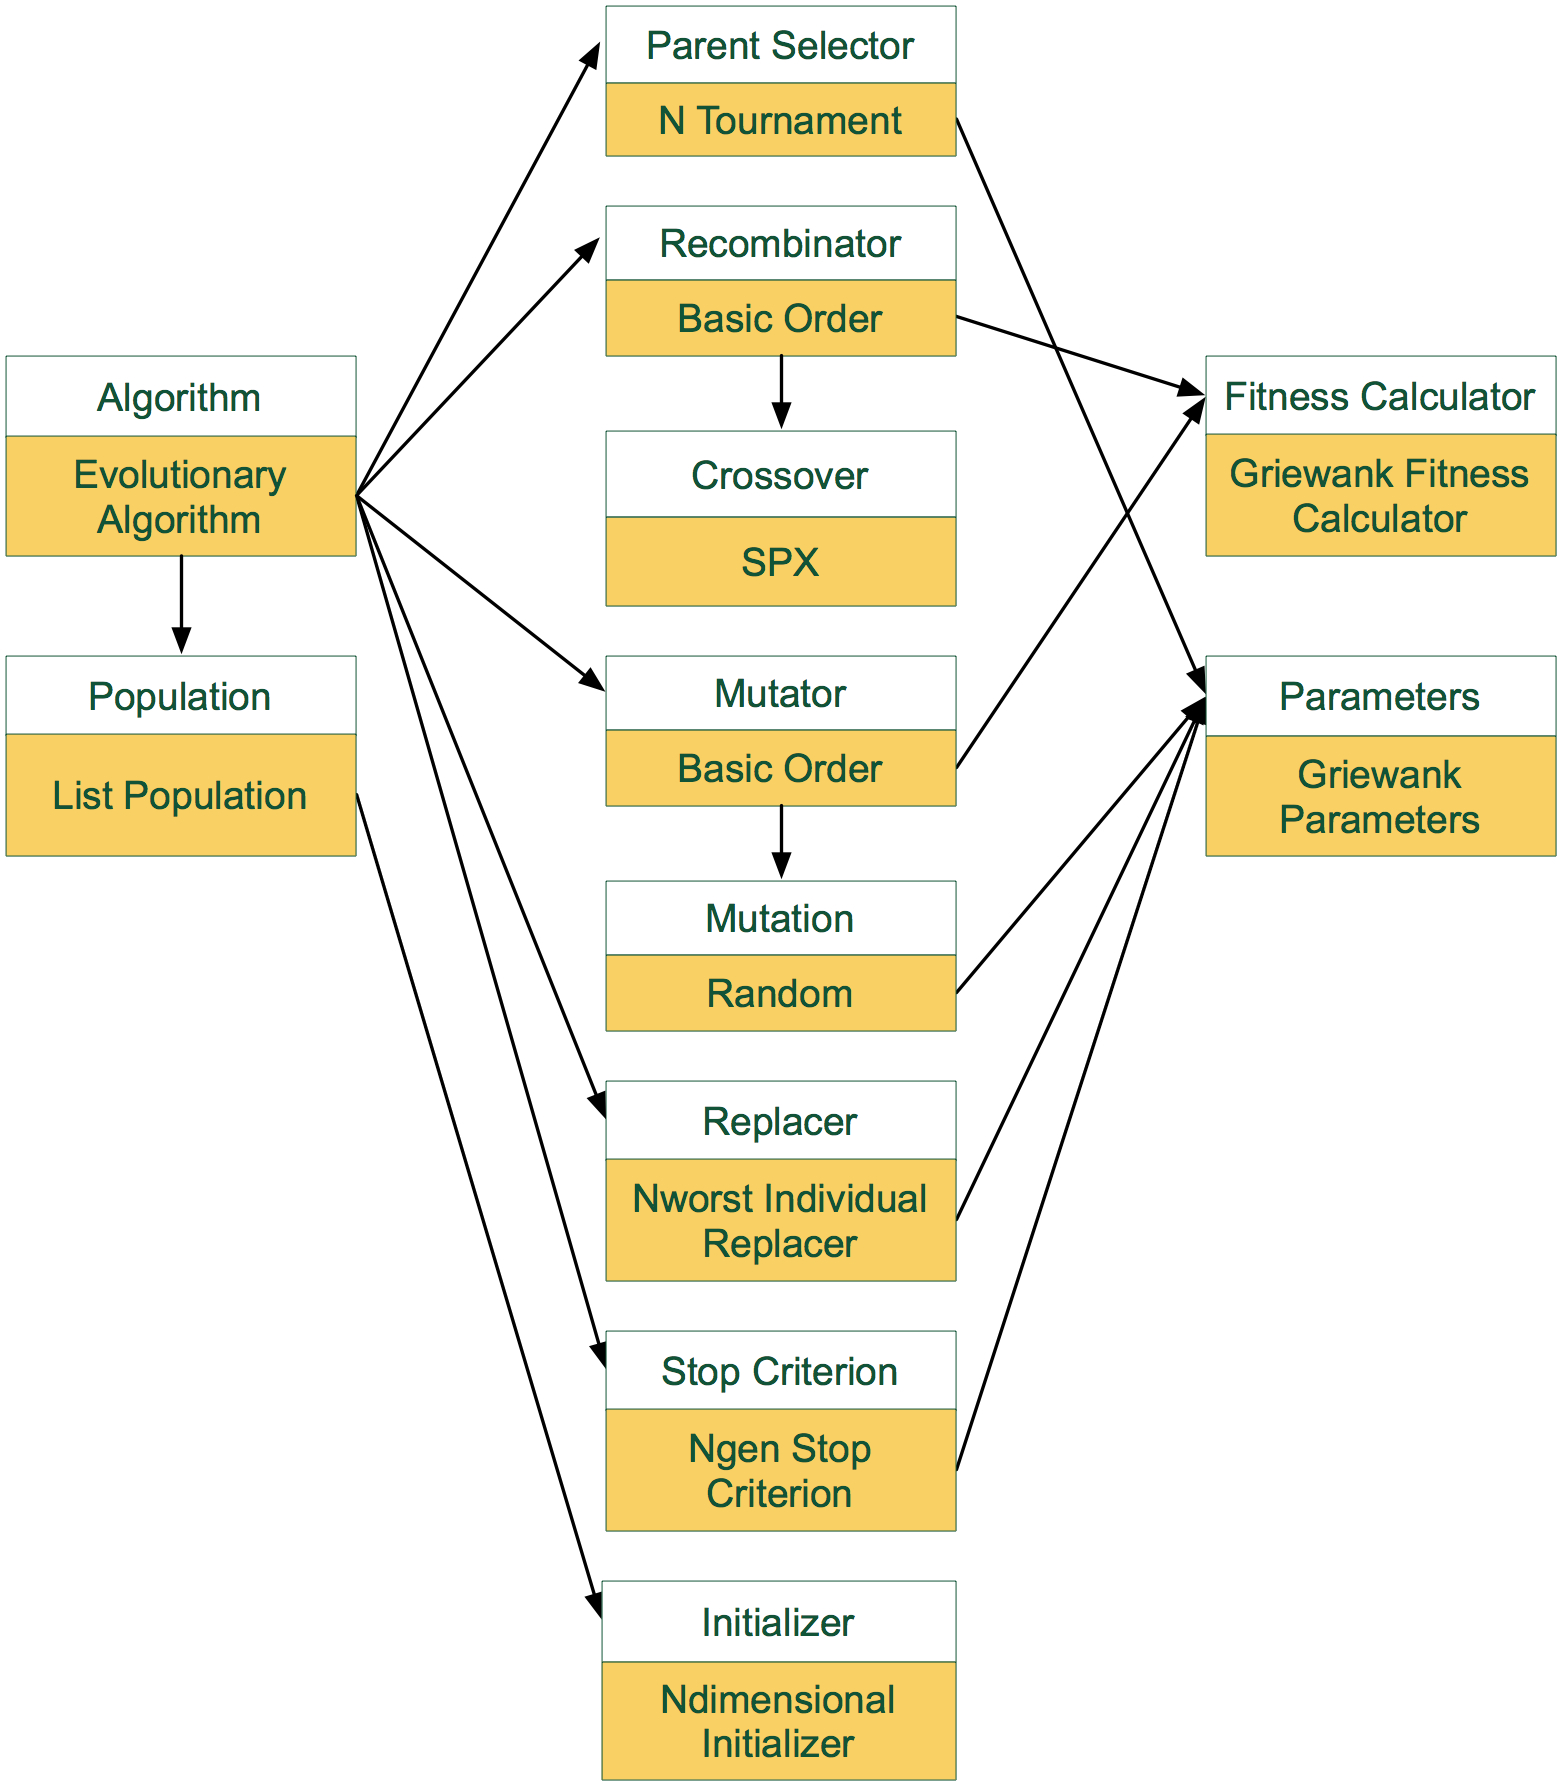
\includegraphics[width=10cm]{gfx/soaea/basicga.jpg}
\caption{Basic genetic algorithm. White blocks are interfaces and orange blocks are implementations. In this case, we are using specific implementations to solve the Griewank function problem.}
\label{BASICGAEXAMPLE}
\end{SCfigure}





Figure \ref{BASICGAEXAMPLE} shows a complete service oriented genetic algorithm, taking into account the proposed ideas. In this figure (and in the following ones) white blocks are the service interfaces. Orange blocks are specific implementations of these interfaces (that is, the source-code of the service), and  arrows indicate how a service implementation can make use of other services via their interface. For example, almost all implementations access to the {\em Parameters} service using its interface. Service implementations (orange blocks) can be selected in a configuration file or be automatically bound when they are available (among other options).

 The change from a problem instance to another is quite simple. It is only necessary to notify the algorithm a change in the implementation of the service {\em Fitness Calculator} and the implementation of {\em Parameters} (because these can vary from a problem to another). Because some algorithms need to calculate the fitness every time an individual is modified (and not only at the end of a generation) the Figure \ref{BASICGAEXAMPLE} shows how the service {\em Fitness Calculator} may be used inside the implementations that modify individuals ({\em Initializer}, {\em Mutator} or {\em Recombinator}). Moreover, each service can be in the local machine or distributed on the Internet, having the same behaviour.

\subsection{Implementing a service oriented NSGA-II}
\label{sec:nsga2}

The difference between the previous version of a GA and the well known NSGA-II \cite{NSGA2} lies in the selection operator. Therefore, to change from the basic GA to NSGA-II, the mutator and crossover are kept and new selection operators are added. Figure \ref{fig:nsga2} shows the service oriented version of NSGA-II algorithm, where the new implementations are marked with a thick border. The problem has also been set to the multi-objective function MOP2 \cite{ReviewMultiobj06}. New auxiliary services have been added, like {\em Crowding Distance Assignator} or {\em Pareto Assignator}. As these services may be used in other algorithms in the future, they must be designed as abstract as possible. These new services are called from the implementation (code) of the services {\em NSGA-II Replacer} or {\em Binary Crowding Distance Selector} (black arrows indicate an interface call). 




\begin{SCfigure}[20][htb]
\centering
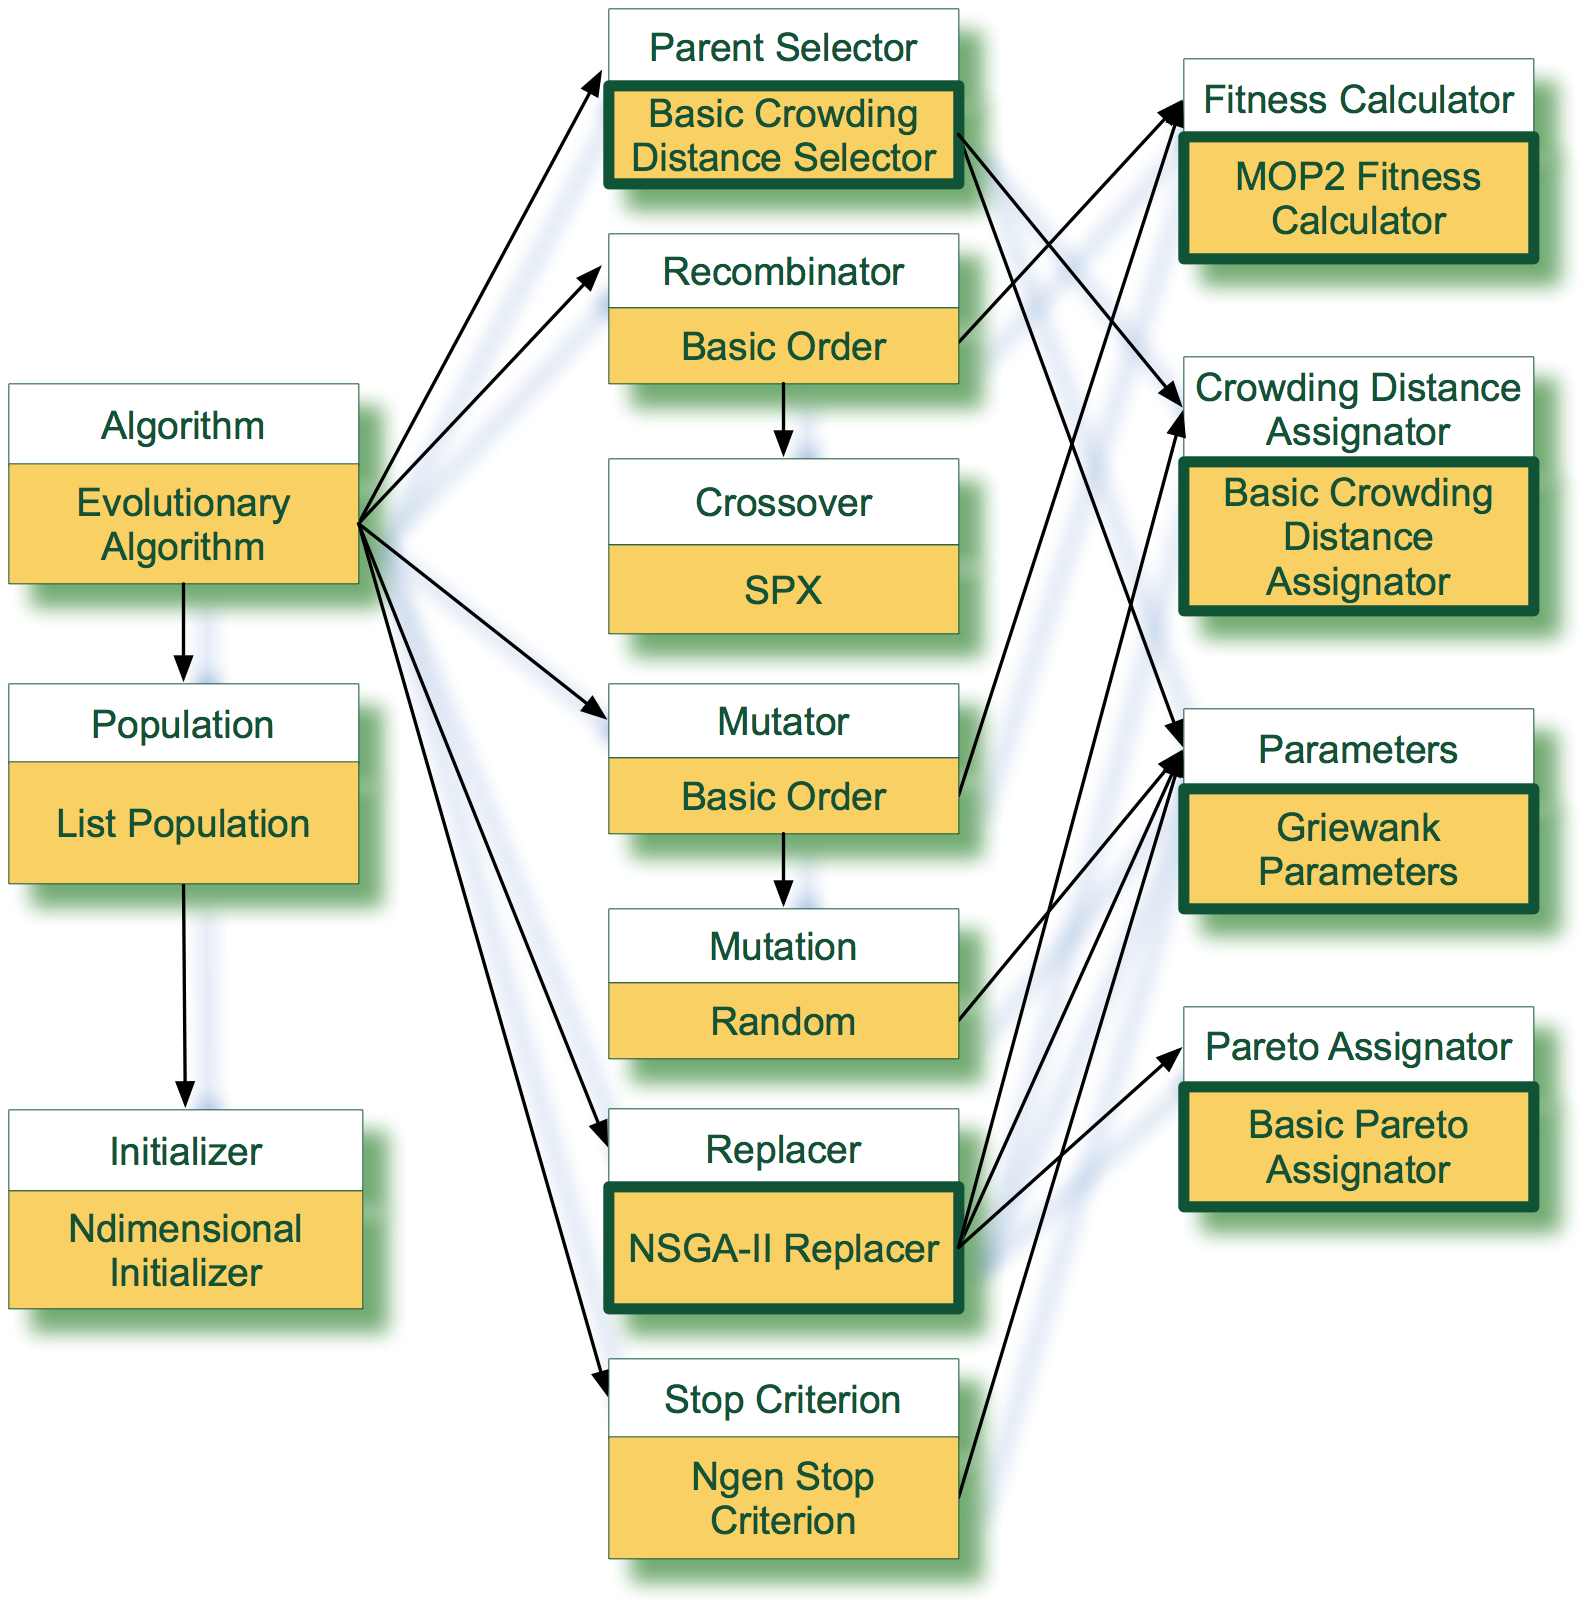
\includegraphics[width=10cm]{gfx/soaea/nsga2.jpg}
\caption{Modification of the basic GA adding new service implementations (orange blocks with thick lines).}
\label{fig:nsga2}
\end{SCfigure}



\subsection{Adding basic distribution}
\label{sec:distribution}

As every service must keep the same behaviour, independently of the machine that hosts it, distribution services for load balancing of a specific service can be easily created, for example, notifying the algorithm to use a distributed implementation for that service. As previously stated, the service {\em Fitness Calculator} receives a list of individuals to calculate their fitness, so, in this example, the new fitness implementation ({\em Basic Fitness Distributor}) binds with every fitness service available (in the same machine or in a network). The source code of this basic implementation simply distributes the list of individuals among the bound services and waits for their termination. Although more complex implementations probably will be more efficient, the objective of this section is to show how to distribute services, thus, this basic implementation is sufficient. Figure \ref{FITNESSDISTRIBUTOR} shows the modification from a sequential fitness calculator to a distributed one. Thanks to SOA, the number of distributed fitness calculators is not fixed: calculators can be added o removed in real time without stopping the system. As can be see in the figure, if one of the nodes is a cluster, it could also  implement another fitness distributor. This easy example can be adapted to more complex necessities depending on the infrastructure or the problem to be solved. More complex distribution services can be created, for example, taking into account communication latencies or computation capabilities of the nodes.




\begin{SCfigure}[20][htb]
\centering
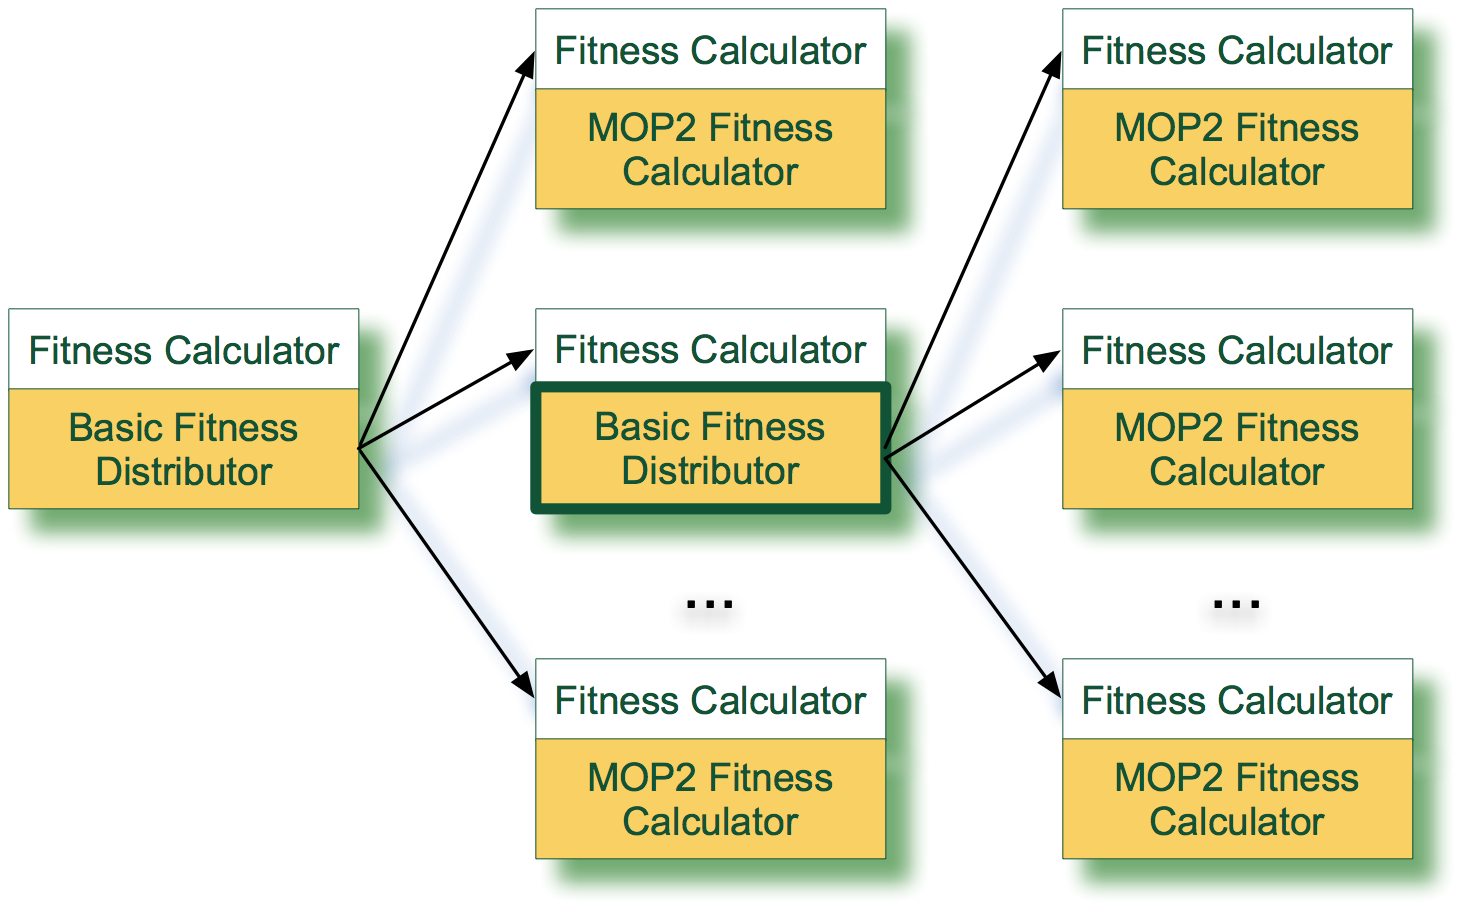
\includegraphics[width=10cm]{gfx/soaea/distributor.jpg}
\caption{Fitness distributor. The thick line implementation also re-distribute the individuals.}
\label{FITNESSDISTRIBUTOR}
\end{SCfigure}



One of the most extended model in parallel EAs is the island model. Using SOA-EA, the {\em Population} service implementation can be modified to become a distributed population. Each certain time, this population could exchange individuals with other populations modified by other algorithms. These populations should be added or deleted in execution time without affecting the algorithm execution. Figure \ref{POPULATION} shows this example, where a Replacer implementations maintains a list of references to other Population interfaces (which can be local or remote). Also other Population implementations exist (List Population is the usual list of individuals). If one of these population services drop, the others can continue working. The topology of these islands can also be managed from services (such as the Basic Replacer service, or another). The  modification and dynamism of the population structure is difficult to apply in existing frameworks without using SOA because it is necessary to create mechanisms to modify the population behaviour, the operators to modify it, the data structures, and also the code to manage all. With he usage of SOA, and due to the capability of accessing to a population via its service interface, it is not necessary to modify the source code to modify the population and its behaviour. Also, to avoid bottlenecks in distributed executions, asynchronous communication must be provided to avoid idle time. This kind of communication offers excellent performance when working with different nodes and operating systems, as demonstrated by \cite{Alba2002Heterogeneous}.



\begin{SCfigure}[20][htb]
\centering
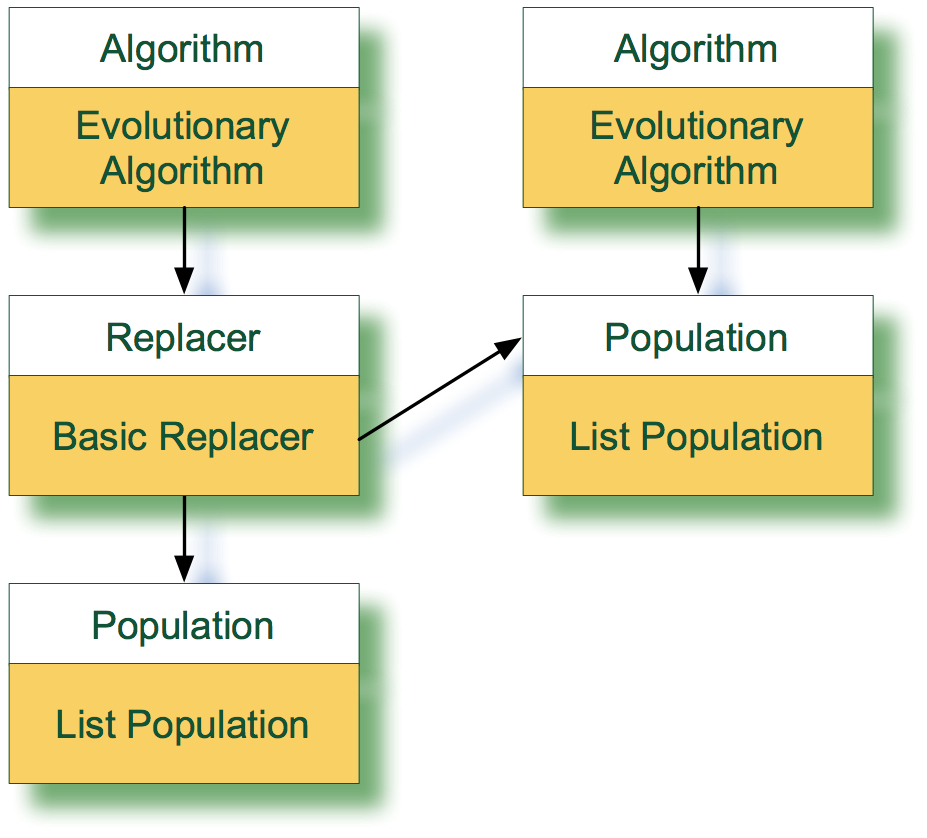
\includegraphics[width=10cm]{gfx/soaea/island.jpg}
\caption{Island model. From time to time, the implementation {\em Island Population} notifies the islands to initiate the migration.}
\label{POPULATION}
\end{SCfigure}



\subsection{Self-adaptation in SOA-EA}
\label{sec:otherexamples}
There are several ways to create self-adaptable algorithms using SOA-EA. For example, creating a service that modifies the parameters in the {\em Parameters} service, or activating and de-activating operators in real time. An easier way is to create a service that manages all available services of the same kind. For example a {\em Mutator} service that binds all the available mutation implementations and use the most adequate one depending on some rules during the execution \cite{SelfadaptationSerpell2010}.  This idea can also be extended to create a service that implements several interfaces and selects the most adequate implementation for each interface respect to some criteria, as can be seen in Figure \ref{INTELLIGENTALGORITHM}, where thick lines represent the implementations used at the current moment (they vary as time passes).



\begin{SCfigure}[20][htb]
\centering
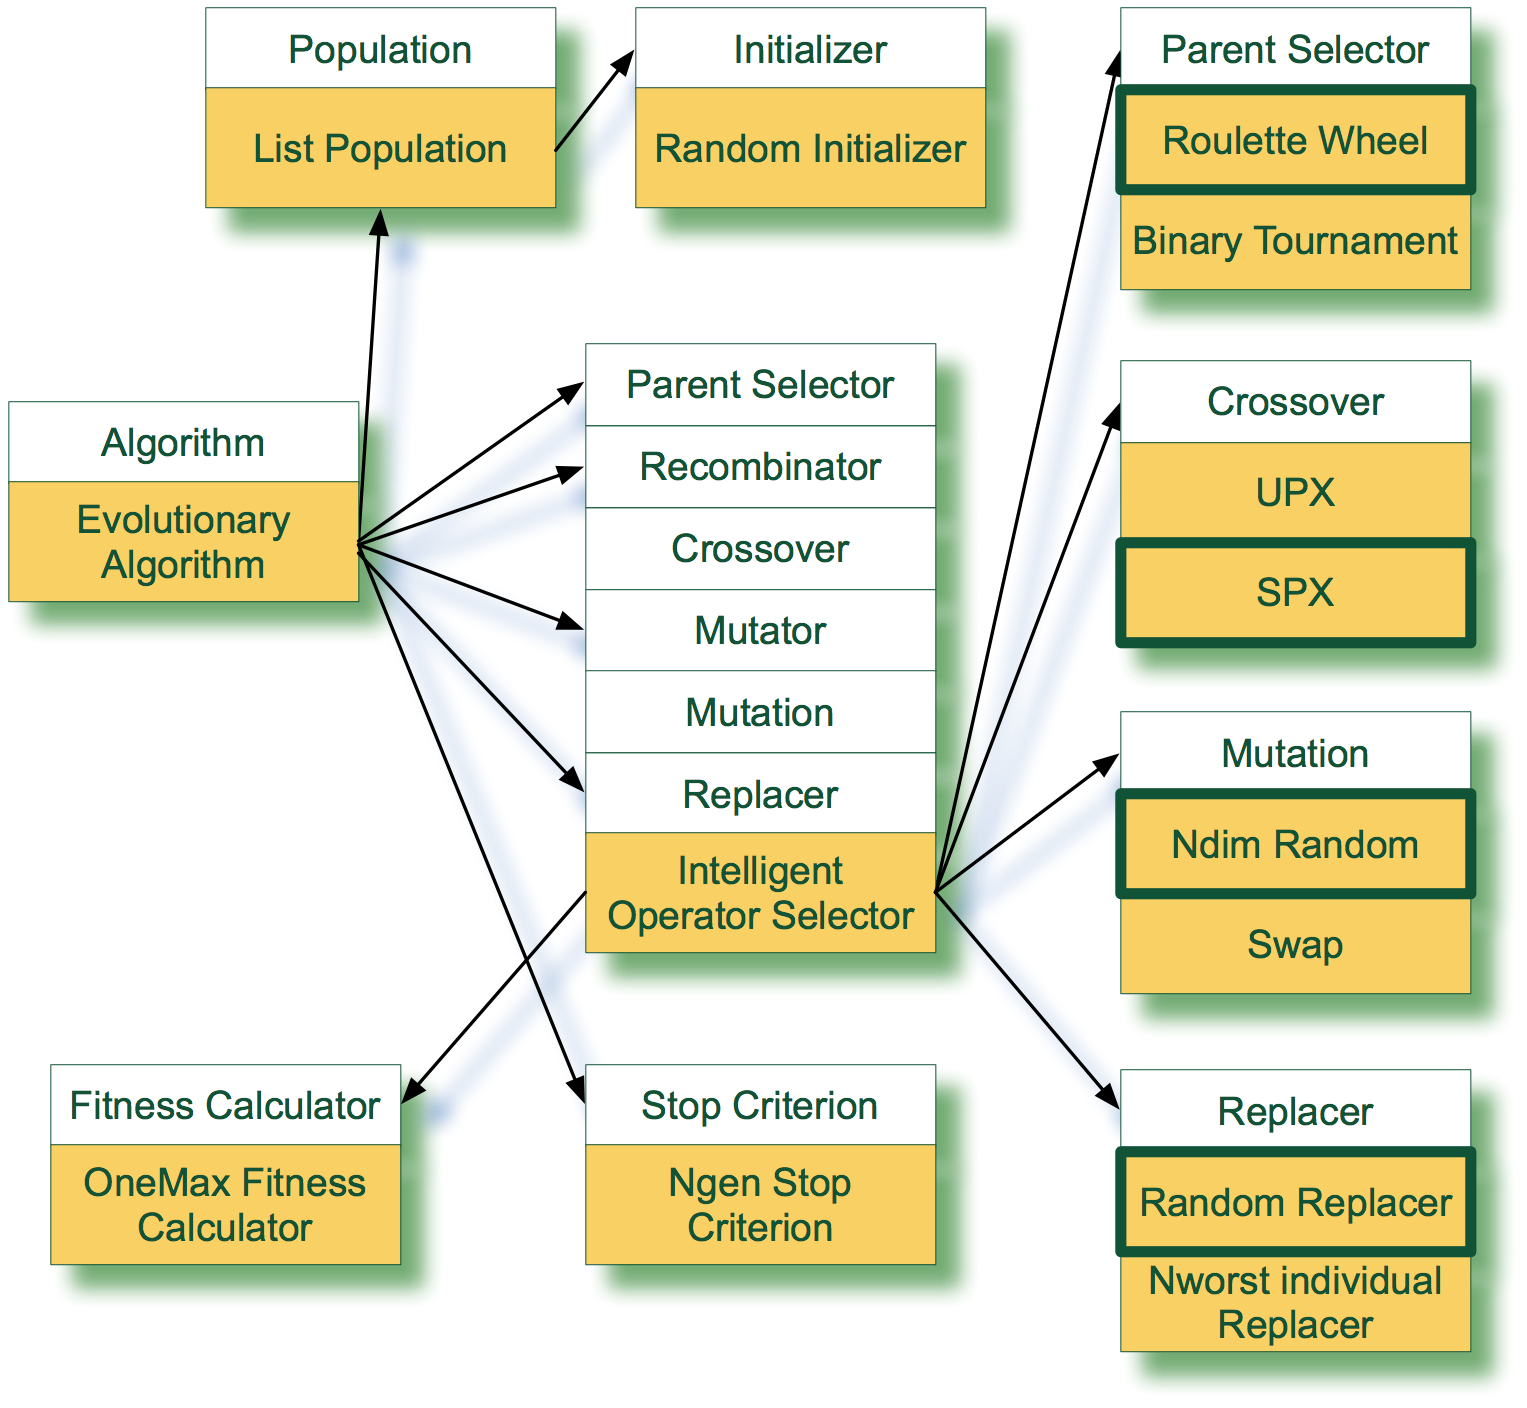
\includegraphics[width=10cm]{gfx/soaea/intelligent.jpg}
\caption{Self-adaptable Algorithm. The {\em Intelligent Operator Selector} selects which service implementation is used each time.}
\label{INTELLIGENTALGORITHM}
\end{SCfigure}


Finally, another important usage of EAs is its hybridization with other metaheuristics, to obtain more effective search algorithms \cite{HybridRodriguez2012},  increasing the performance of intensification and diversification mechanisms. With  traditional frameworks this task can be difficult, mainly because the source code for each metaheuristic must be modified. Nevertheless, using SOA a combination of loosely coupled services could be used.

